\documentclass[12pt, twoside]{article}
\usepackage[letterpaper, margin=1in, headsep=0.5in]{geometry}
\usepackage[english]{babel}
\usepackage[utf8]{inputenc}
\usepackage{amsmath}
\usepackage{amsfonts}
\usepackage{amssymb}
\usepackage{tikz}
%\usetikzlibrary{quotes, angles}

\usepackage{graphicx}
\usepackage{enumitem}
\usepackage{multicol}

\usepackage{fancyhdr}
\pagestyle{fancy}
\fancyhf{}
\renewcommand{\headrulewidth}{0pt} % disable the underline of the header

\fancyhead[R]{\thepage}
\fancyhead[L]{BECA / Dr. Huson / 10th Grade Geometry\\* Learning trajectory: Segments}

\begin{document}
\subsubsection*{Segment addition and partition}
\begin{enumerate}
  \item Segment addition
  \item Midpoint calculation
  \item Midpoint on the $x$-$y$ plane
  \item Ratio partition
  \item Applied to triangle legs
  \end{enumerate}

\begin{enumerate}
\subsubsection*{Segment addition short questions}
  \item Given $\overline{ABC}$, $AC=5 \frac{1}{3}$, and $BC=1$.
    \begin{enumerate}
      \item Find ${AB}$.\\[0.75cm]
        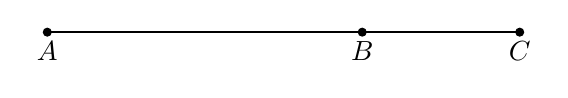
\begin{tikzpicture}
          \draw [-, thick] (1,0)--(7,0);
          \draw [fill] (1,0) circle [radius=0.05] node[below]{$A$};
          \draw [fill] (5,0) circle [radius=0.05] node[below]{$B$};
          \draw [fill] (7,0) circle [radius=0.05] node[below]{$C$};
        \end{tikzpicture} \bigskip
      \item The postulate used in this problem is the \rule{6cm}{0.15mm}.
      \end{enumerate}

\subsubsection*{Midpoint short questions}
  \item Given $\overleftrightarrow{QS}$ as shown on the number line. \\[10pt]
    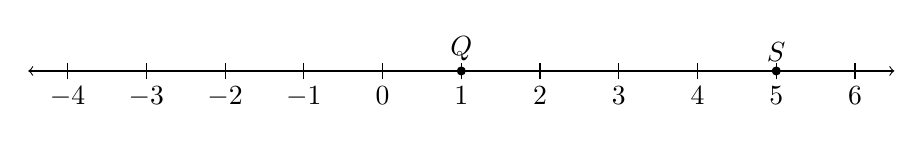
\begin{tikzpicture}
      \draw [<->] (-4.5,0)--(6.5,0);
      \foreach \x in {-4,...,6} %2 leading for diff!=1
        \draw[shift={(\x,0)},color=black] (0pt,-3pt) -- (0pt,3pt) node[below=5pt]  {$\x$};
        \draw [fill] (1,0) circle [radius=0.05] node[above] {$Q$};
        \draw [fill] (5,0) circle [radius=0.05] node[above] {$S$};
    \end{tikzpicture}
    \begin{enumerate}
      \item Mark the point $R$, the midpoint of $\overline{QS}$.
      \item The point $P$ is collinear with $\overleftrightarrow{QS}$ such that $Q$ is the midpoint of $\overleftrightarrow{PS}$. Mark $P$ on the line.
      \end{enumerate}

\subsubsection*{Midpoint on the $x$-$y$ plane}
  \item In the diagram below, $\overleftrightarrow{AC}$ has endpoints with coordinates $A(-3,2)$ and $C(3, -7)$.
    \begin{center} %4 quadrant regents grid
    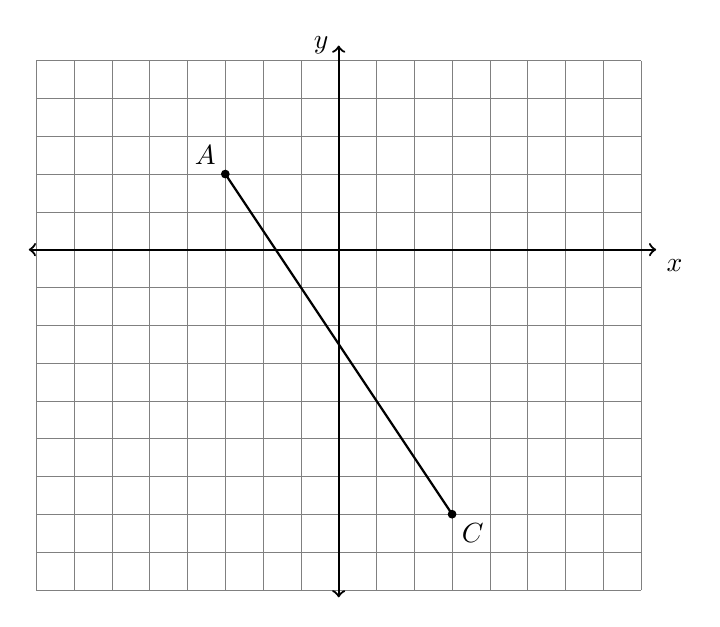
\begin{tikzpicture}[scale=.48]
      \draw [help lines] (-8,-9) grid (8,5);
      \draw [thick, <->] (-8.2,0) -- (8.4,0) node [below right] {$x$};
      \draw [thick, <->] (0,-9.2)--(0,5.4) node [left] {$y$};
      \draw [thick] (-3,2)--(3,-7);
      \draw [fill] (-3,2) circle [radius=0.1] node[above left] {$A$};
      \draw [fill] (3,-7) circle [radius=0.1] node[below right] {$C$};
    \end{tikzpicture}
    \end{center}
    If $B$ is a point on  and $AB {:} BC = 1{:}2$,  what  are  the  coordinates
of $B$?


\subsubsection*{Segment addition algebra}
  \item Given collinear points $P, Q, R$ with $Q$ bisecting the line segment $\overline{PR}$. $PQ=x-2$ and $QR = \frac{1}{2} x+6$. Find the length of $\overline{PR}$.\\ \bigskip
    First label the drawing.
    \begin{flushright}
    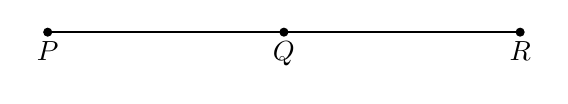
\begin{tikzpicture}
      \draw [-, thick] (0,0)--(6,0);
      \draw [fill] (0,0) circle [radius=0.05] node[below]{$P$};
      \draw [fill] (6,0) circle [radius=0.05] node[below]{$R$};
      \draw [fill] (3,0) circle [radius=0.05] node[below]{$Q$};
    \end{tikzpicture}
    \end{flushright}
    %\vspace{1cm}
    \begin{enumerate}
      \item Write a geometric equation: \rule{4cm}{0.15mm} \hspace{1cm} \rule{4cm}{0.15mm}
      %\vspace{.7cm}
      \item Substitute algebraic values: \rule{4cm}{0.15mm}
      \item Solve for $x$
      %\vspace{4.5cm}
      %\begin{center} $x=$ \rule{1cm}{0.15mm} \end{center}
      \item Answer the question:
      %\vspace{2.5cm}
      \item Check your answer
    \end{enumerate}

    \item \emph{variation} Given collinear points $P, Q, R$ with $Q$ bisecting the line segment $\overline{PR}$. $PQ=\frac{1}{2} x+4$ and $PR = 4x$. Find the length of $\overline{PR}$.



  \end{enumerate}
\end{document}
